% ****** Start of file apssamp.tex ******
%
%   This file is part of the APS files in the REVTeX 4.1 distribution.
%   Version 4.1r of REVTeX, August 2010
%
%   Copyright (c) 2009, 2010 The American Physical Society.
%
%   See the REVTeX 4 README file for restrictions and more information.
%
% TeX'ing this file requires that you have AMS-LaTeX 2.0 installed
% as well as the rest of the prerequisites for REVTeX 4.1
%
% See the REVTeX 4 README file
% It also requires running BibTeX. The commands are as follows:
%
%  1)  latex apssamp.tex
%  2)  bibtex apssamp
%  3)  latex apssamp.tex
%  4)  latex apssamp.tex
%
\documentclass[
 reprint,
%superscriptaddress,
%groupedaddress,
%unsortedaddress,
%runinaddress,
%frontmatterverbose, 
%preprint,
%showpacs,preprintnumbers,
%nofootinbib,
%nobibnotes,
%bibnotes,
 amsmath,amssymb,
 %aps,
pra,
%prb,
%rmp,
%prstab,
%prstper,
%floatfix,
]{revtex4-1}

\usepackage{graphicx}% Include figure files
\usepackage{dcolumn}% Align table columns on decimal point
\usepackage{bm}% bold math
% \usepackage{hyperref}% add hypertext capabilities
%\usepackage[mathlines]{lineno}% Enable numbering of text and display math
%\linenumbers\relax % Commence numbering lines

%\usepackage[showframe,%Uncomment any one of the following lines to test 
%%scale=0.7, marginratio={1:1, 2:3}, ignoreall,% default settings
%%text={7in,10in},centering,
%%margin=1.5in,
%%total={6.5in,8.75in}, top=1.2in, left=0.9in, includefoot,
%%height=10in,a5paper,hmargin={3cm,0.8in},
%]{geometry}


\begin{document}


\title{Quantum-like behavior at Macroscopic Scale (Analysis)}% Force line breaks with \\
% \thanks{A footnote to the article title}%

\author{Marcel Reis Soubkovsky}
 \email{marcel.soubkovsky4@etu.univ-lorraine.fr}
\affiliation{%
 University of Lorraine, Master's in Applied Physics and Physics Engineering
}%

\date{\today}% It is always \today, today,
             %  but any date may be explicitly specified

\begin{abstract}
% An article usually includes an abstract, a concise summary of the work
% covered at length in the main body of the article. 
Write this at last

\end{abstract}

\maketitle

%\tableofcontents

When imagining a drops colliding with an interface of the same fluid it is acceptable to assume that the drop will merge with the fluid in order to minimize the surface area.
While doing experiments with soap solutions under vertical vibration, J. Walker observed that the solution could keep a stable drop floating on the surface of the fluid.\cite{walker_drops_nodate}
A bath filled with a fluid can hold a droplet of the same fluid when put into vertical vibration of surface acceleration greater than $g$.\cite{couder_bouncing_2005}
 \\
(img 1)
\\
The droplet is kept bouncing over the fluid and is then free to move horizontally due to vertical stabilization. At first, this horizontal movement seemed very random. Couder and Fort first noticed that the random nature of the horizontal movement of the droplet could be described by diffraction and interference waves.\cite{couder_single-particle_2006}. During a series of experiments, Couder and Fort placed a single slit on the vibrating bath. After successive repetitions, the final positions of the droplet described a diffraction wave.
\\
(img 2)
\\



\section{Similarities between light diffraction patterns and the droplet diffraction}

	\begin{figure}[h]
		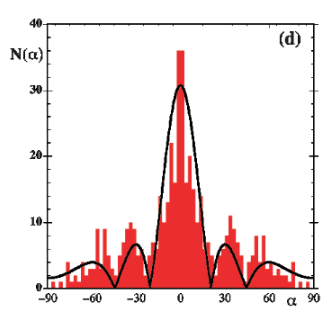
\includegraphics[width=0.25\textwidth]{img2.png}
		\caption{Histogram obtained by Couder and Fort using a slit of width $L=14.8$mm and a Faraday wavelength of $\lambda_F = 6.95$mm \cite{couder_single-particle_2006}}
		\label{fig:diffraction}
	\end{figure}

	\subsection{Fraunhofer diffraction theory}
    
    The diffraction pattern curve provides an approximate fit to the histogram found by Couder and Fort's experiments. In Fraunhofer Wave Optics, the diffraction pattern can be observed when a beam of light passes through a narrow slit. If a screen is placed at a certain distance from the slit, a Fraunhofer diffraction pattern can be observed on the screen.\cite{serway_physics_2014} The pattern drawn by light is the one show in figure \ref{fig:diffraction}. The intensity can be calculated using the following formula
    $$ I=I_{max} \left[ \frac{\sin (\pi a \sin \theta / \lambda)}{\pi a \sin \theta / \lambda} \right]^2$$
    where $I_{max}$ is the intensity at $\theta=0$,$a$ is the length of the slit,$\theta$ is the angle of deviation after the slit and $\lambda$ is the wavelength of the beam. The expression can be simplified when considering only the position of the minima. The condition for intensity minima on a single slit problem states that

    $$ \frac{\pi a \sin \theta_{minima}}{\lambda}=m\pi$$
    or
    $$ \sin \theta_{minima}=m \frac{\lambda}{a} $$

    where $ m=\pm 1, \pm 2, \pm 3, \dots$

    \subsection{Couder and Fort's approximation}

    The histogram produced after several trials with the vibrating bath single slit setup could be compared to a diffraction wave produced by a Fraunhofer diffraction as shown in figure \ref{fig:diffraction}. Couder and Fort approximated the formula for the intensity of a Fraunhofer diffraction pattern to the pattern drawn by the final position of the droplet. The function for this specific problem in diffraction of a droplet can be represented as

    $$ f(\alpha) = A \left|\frac{\sin{(\pi L \sin{\alpha}/\lambda_F)}}{\pi L \sin{\alpha}/\lambda_F}\right|$$

    where $A$ is the maximum amplitude, $L$ is the width of the slit and $\alpha$ the deviation angle of the droplet after the slit.


\section{Similarities between light interference patterns and the droplet histogram}

	Couder and Fort proceeded then to study the possibility of producing an interference pattern with the vibrating bath system that was built for the study of the single slit diffraction. The single slit was replace by a double slit in order to reproduce Young's double slit experiment with a droplet on a vibrating bath. The droplet drew clear interference fringes that are well fitted by the following formula:

	$$f(\alpha)=A \left|\frac{\sin{(\pi L \sin{\alpha}/\lambda_F)}}{\pi L \sin{\alpha}/\lambda_F} \cos{(\pi d \sin{\alpha}/\lambda_F)}\right|$$

	where $d$ is the distance between the centers of the slits.

	In the domain of wave optics, the interference produced by a double slit diffraction pattern is given by the expression:

	$$I=I_{max} \cos ^2 \left(\frac{\pi d \sin \theta}{\lambda}\right) \left[ \frac{\sin (\pi a \sin \theta / \lambda)}{\pi a \sin \theta / \lambda}\right]^2$$

	\begin{figure}
		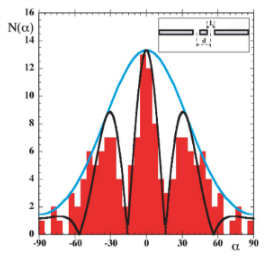
\includegraphics[width=0.30\textwidth]{img3.png}
		\caption{Histogram for the deviation of 75 particles through two slits of width $L = 7.6$ mm, a distance $d = 14.3$ mm apart, the droplet's wavelength being $\lambda_F = 6.95$ mm ($L/\lambda_F = 1.1$ and $d/\lambda_F = 1.87$). The blue(light) line is the envelope due to the diffraction of a single slit while the curve in black is the optimum fit by the equation that is based on the interference pattern obtained for effective values $L/\lambda_F = 0.9$ and $d/\lambda_F = 1.7$. Source:\cite{couder_single-particle_2006}}
		\label{fig:interference}
	\end{figure}

	The approximation fits closely as shown in figure \ref{fig:interference}. This brought up many questions concerning the physical engine behind this phenomenon. The conclusions Couder and Fort brought are discussed further on. %add internal link

\section{Quantum-like behavior}
	
	% The vibrating bath with a droplet that was free to move horizontally was then studied on a circular corral by Harris, Moukhtar, Fort, Couder and Bush \cite{harris_wavelike_2013}.
	Oh my god
	



    % \subsection{Experimental Apparatus used by Harris, Moukhtar, Fort, Couder, and Bush}


% \section{Similarities to Quantum Phenomena}

    % \subsection{Patterns formed by free moving droplets}
    % \subsection{Diffraction and Interference of bouncing droplet}
    %     \subsubsection{Single and Double Slit}
    % \subsection{Circular Corral}
    
    
    
    \bibliographystyle{plain}
    
    \bibliography{bibtex}



\end{document}